% To make a PDF from this source, use the pdflatex command.
\documentclass[helvetica,english,utf8,notitle,nologo]{beamer}
\usetheme{default}
\usecolortheme{seahorse}
\usepackage{graphicx}
\graphicspath{ {images/} }

\begin{document}

\title{Intro to Ansible}
\author{Carlos Konstanski}

\frame{\titlepage}

\begin{frame}
  \frametitle{Presentation Materials Available Online At:}
  \href{url}{https://github.com/ckonstanski/ansible-presentation}
\end{frame}



\begin{frame}
  \frametitle{Configuration Management In General}

  Ansible is a configuration management system. Some other popular
  examples are Puppet, Chef and Salt.

  A configuration management system allows you to automate the
  installing and configuration of software on computers. It doesn't
  matter what the computers are used for. They could be servers or
  workstations. They could be baremetal or virtual machines. We use
  the generic term ``nodes'' to talk about the computers that are the
  targets (or ``clients'') of configuration management.

  These are some of the benefits of using configuration management:

  \begin{itemize}
  \item Labor- and time-saving
  \item Defined in software; business logic can be applied
  \item Distro-specific details abstracted away
  \item Idempotency
  \item The person who writes the configuration management doesn't
    have to be the person who runs it
  \end{itemize}
\end{frame}

\begin{frame}
  \frametitle{Idempotency}

  An idempotent operation has the following characteristics:

  \begin{itemize}
  \item Only performs an action if the node is not in the state that
    the operation is meant to achieve
  \item Can be run any number of times without damaging the state of
    the node
    \begin{itemize}
    \item Example: insert vs. upsert
    \item Example: append vs. lineinfile
    \end{itemize}
  \end{itemize}
\end{frame}

\begin{frame}
  \frametitle{Configuration Management Architecture: Server and Targets}

  Most configuration managements use a two-tier architecture. There is
  a central server node (called a server, master or control node
  depending on the configuration management product in use) and any
  number of target nodes (called targets or clients). The
  configuration definitions live on the server and get transmitted to
  the targets via either a push or pull mechanism.
\end{frame}

\begin{frame}
  \frametitle{Pull-Type Systems}

  In a pull-type system, each target has an agent running on
  it. Periodically the agent wakes up and connects to the server to
  pull the latest configuration and apply it. Chef and Puppet are
  examples of this type of architecture.

  Pull-type systems are great when you want targets to keep themselves
  updated automatically. You just need to update the configuration on
  the server and wait for the targets to check in.

  Running a configuration management tool against a target to bring
  its configuration up to date is often referred to as bringing the
  target into convergence. This term is especially popular in the Chef
  world.
\end{frame}

\begin{frame}
  \frametitle{Push-Type Systems}
  
  In a push-type system, there still has to be something on each
  target that enables a connection from the server. But it is the
  server that initiates the connection. Salt and Ansible are examples
  of this type of architecture. Salt uses a ZeroMQ queue to
  transmit data. Ansible uses SSH.

  Push-type systems are better when you want to control when the
  targets receive updates. The targets aren't automatically checking
  in on a periodic schedule. You have to ``push a button''.
\end{frame}

\begin{frame}
  \frametitle{Asynchronous Convergence vs. Orchestration}

  Pull-type systems like Chef and Puppet are geared toward configuring
  each target as an island unto itself. Since each target checks in
  asynchronously with respect to the other targets, any given target
  cannot know what is happening on other targets, and there is no way
  to instruct the system to converge targets in a particular order.

  Since Ansible is a push-type system, it has the inherent ability to
  configure an entire stack of targets in a coordinated manner. The
  order in which operations are pushed to targets is under full
  control. This makes Ansible a true orchestration tool.

  In the enterprise you will often find both a client-server system
  like Chef or Puppet and an an orchestration system like Ansible or
  Salt in use. Both types of problems need to be solved, and it takes
  both tools to provide coverage.
\end{frame}

\begin{frame}
  \frametitle{Supported Platforms}

  The Ansible server must be a *NIX running Python. (Python3 support
  has been recently added) Many Linux distros, Mac OSX and *BSD are
  viable options, and there may be a few others as well (Solaris?).

  There are very few moving parts to Ansible. It's just a python
  app. You don't need a dedicated server. Any laptop will do. There
  are no daemons or listeners on the server. The listeners are the SSH
  daemons running on the targets.

  The targets can run any OS that can be configured to respond to SSH
  connections. However each Ansible ``resource'' that you use must be
  able to handle the OS of the target. This support is coded into each
  resource individually. They say that Windows is supported, but I
  have never tried it. Certainly any OS that is supported on the
  control node is also supported on the targets (e.g. *NIX).
\end{frame}

\begin{frame}
  \frametitle{Configuring Connections to Targets}

  The master configuration on the control node resides in two files:
  /etc/ansible/ansible.cfg and /etc/ansible/hosts. In addition every
  target requires passwordless SSH configuration.
\end{frame}

\begin{frame}
  \frametitle{ansible.cfg}

  ansible.cfg defines defaults for the options that control many
  aspects of how ansible runs. It is written in INI format. The
  following is a short but very typical example:

  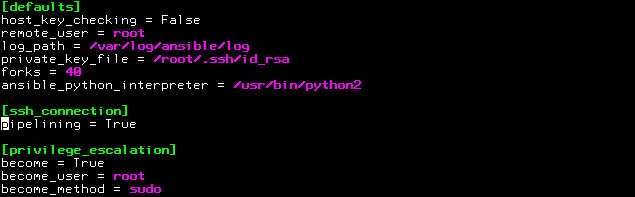
\includegraphics[scale=0.44]{img_1}

  ansible.cfg can be located in various places. Here is the order of
  precedence:

  \begin{itemize}
  \item ANSIBLE\_CONFIG (an environment variable)
  \item ansible.cfg (in the current directory)
  \item .ansible.cfg (in the home directory)
  \item /etc/ansible/ansible.cfg
  \end{itemize}
\end{frame}

\begin{frame}
  \frametitle{hosts}

  The Ansible hosts file defines names for target groups. Each group
  contains the names of the targets belonging to that group. Each
  target can have options that override the defaults in
  ansible.cfg. Like ansible.cfg it is written in INI format.

  The target names must be resolvable by SSH. More on this later.

  By default the hosts file is located at /etc/ansible/hosts. You can
  add the -i option to your ansible or ansible-playbook command to
  point to another location.

  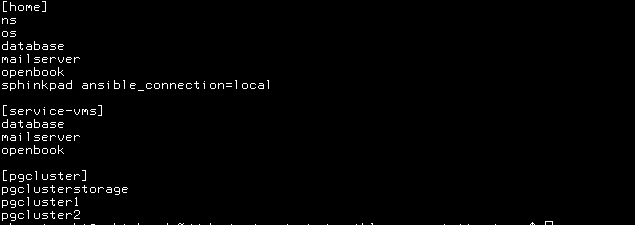
\includegraphics[scale=0.44]{img_2}
\end{frame}

\begin{frame}
  \frametitle{\textasciitilde/.ssh/config}

  In order to fully understand the target names in the ansible hosts
  file, a complete picture must be built taking both DNS and the SSH
  config into account. Look in /etc/ssh/ssh\_config and
  \textasciitilde/.ssh/config for all such SSH entries. The following
  is a typical \textasciitilde/.ssh/config file:

  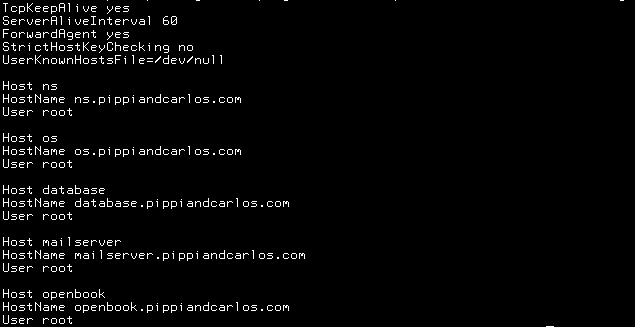
\includegraphics[scale=0.44]{img_3}
\end{frame}

\begin{frame}
  \frametitle{authorized\_keys}

  In order for the server to be able to SSH onto the targets without a
  password, the server's SSH public key must be installed on the
  targets. The configuration option private\_key\_file in ansible.cfg
  points to the private key that ansible will use when making
  connections. The corresponding public key must be copied to the
  targets.

  Where does the public key go on the target? Look at remote\_user in
  ansible.cfg. This is the user that ansible will attempt to use in
  the SSH connection. This user must exist on the target. In that
  user's home directory on the target will be an .ssh/authorized\_keys
  file. That's where the public key gets added.

  If the authorized\_keys file does not exist, create it. Use
  ssh-keygen to create the .ssh directory (if it doesn't already
  exist), and then create the authorized\_keys file manually.
\end{frame}

\begin{frame}
  \frametitle{Two Modes of Operation: Ad-Hoc and Playbook}

  Ansible can be used in two ways:

  \begin{itemize}
  \item Ad-Hoc
    \begin{itemize}
    \item Typed into a terminal; not read from a file
    \item Runs a single command
    \item Command: ansible
    \end{itemize}
  \item Playbook
    \begin{itemize}
    \item Read from a file or collection of files
    \item Runs any number of commands in a deterministic order
    \item Command: ansible-playbook
    \end{itemize}
  \end{itemize}
\end{frame}

\begin{frame}
  \frametitle{Ad-Hoc}

  Ad-hoc Ansible is used when you want to run a single action against
  a target group from a command prompt. Two common actions are: ping
  and shell. Examples of both will follow. Ad-Hoc commands are not run
  from a file; they are typed in at the command prompt. They are
  ephemeral.

  Use the ``ansible'' command to run ad-hoc Ansible.
\end{frame}

\begin{frame}
  \frametitle{Ad-Hoc Example: Ping}

  The ping resource is perhaps the simplest to use. It simply checks
  to see if a target is up and responding to Ansible's SSH
  connection. Note that this is not an ICMP ping. Ansible is actually
  SSHing to the target and invoking python (specifically the python
  executable specified in your ansible.cfg or overridden by your
  inventory). The SSH connection must be correctly configured and
  python must be installed on the target in order for ping to return
  successfully.

  
\includegraphics[scale=0.44]{img_4}
\end{frame}

\begin{frame}
  \frametitle{Ad-Hoc Example: Shell}

  The shell resource is incredibly useful in both ad-hoc and playbook
  applications. It runs an arbitrary shell command on the target.

  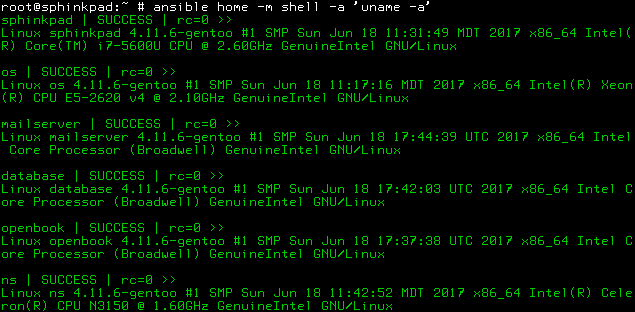
\includegraphics[scale=0.44]{img_5}
\end{frame}

\begin{frame}
  \frametitle{Playbook}

  Ad-hoc ansible is great for ad-hoc situations, and you'll use it a
  lot. But you also want to be able to write playbooks to take
  advantage of the following benefits:

  \begin{itemize}
  \item Far more complex configurations are possible
  \item Saved to files so you can run them easily, save them to git,
    etc.
  \end{itemize}

  Use the ``ansible-playbook'' command to run Ansible playbooks.
\end{frame}

\begin{frame}
  \frametitle{Playbook: Definition}

  An Ansible playbook is a collection of files that Ansible reads,
  parses and executes to bring a specific groups of targets into
  convergence with a specific configuartion. Three types of files make
  up an Ansible playbook:

  \begin{itemize}
  \item Playbook configration files (YAML)
  \item Static files to be copied to targets (any file type)
  \item Jinja templates for dynamically generating files to be copied
    to targets (any \textit{text} file type)
  \end{itemize}
\end{frame}

\begin{frame}
  \frametitle{Playbook: Directory Structure}

  There is a convention for organizing the directory structure of a
  playbook. The top-level of the playbook should contain the following
  directories:

  \begin{itemize}
  \item playbooks (for the YAML files that define the configuration)
  \item roles (for tasks and variables that match a hosts designation)
  \item templates (for jinja templates)
  \item files (for static files)
  \end{itemize}
\end{frame}

\begin{frame}
  \frametitle{Playbook Example: Ping}

  This minimal playbook is analogous to the ad-hoc ping example given
  earlier:

  
\includegraphics[scale=0.44]{img_6}
\end{frame}

\begin{frame}
  \frametitle{Playbook Example: Ping}

  And here is its invocation:

  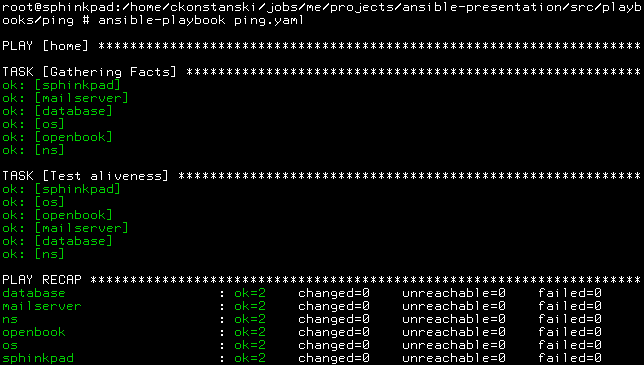
\includegraphics[scale=0.44]{img_7}
\end{frame}

\begin{frame}
  \frametitle{Logic}

  Ansible supports two features that give it the power of a
  programming language: variables and Jinja templating. Without these
  features Ansible would be nothing more than a way to automate
  hardcoded commands. But with these features a whole new dimension of
  power is introduced. Decisions can be made at runtime. Targets can
  be configured dynamically and programatically.
\end{frame}

\begin{frame}
  \frametitle{Logic}

  A few examples to whet your whistle:

  \begin{itemize}
  \item You can give targets hostnames that reflect what kind of
    server it should be. Ansible can parse the hostname and decide
    what to do to the target based on the information therein.
  \item You can write any arbitrary shell logic that returns a value
    and assigns it to a variable. For instance you can run an eyaml
    command in a shell resource to get a password or other secret from
    a Puppet encrypted YAML file, assign that value to a variable, and
    use that variable throughout your Ansible playbook.
  \item You can use an external program to write custom Ansible
    inventory JSON (more on this later). Variables can be fed into a
    playbook via the inventory.
  \end{itemize}
\end{frame}

\begin{frame}
  \frametitle{Variables}

  Variables can be introduced into the playbook at many different
  points:

  \begin{itemize}
  \item Facts
  \item Inventory
  \item Command line: --extra-vars
  \item ``vars'' attribute of a playbook header
  \item ``with\_items'' attribute of a playbook resource
  \item ``register'' attribute of a playbook resource
  \end{itemize}
\end{frame}

\begin{frame}
  \frametitle{Facts}

  All configuration management systems have a means of gathering
  information from the targets and making that data available to the
  configurations that you write. Ansible calls these data
  ``facts''. (Puppet uses the same terminology; Chef calls them
  ``attributes'', Salt calls them ``grains''.)

  Ansible runs a resource called ``setup'' against the target to
  obtain its facts. The result is a rather large JSON blob. Here is a
  tiny snippet:

  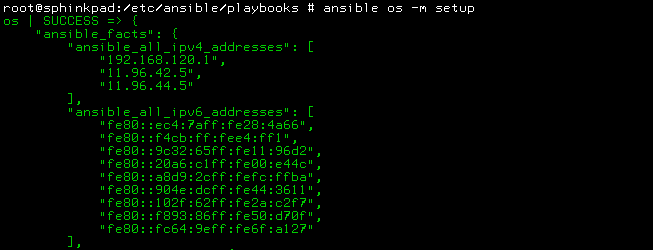
\includegraphics[scale=0.44]{img_8}
\end{frame}

\begin{frame}
  \frametitle{Inventory}

  Technically speaking, the Ansible inventory is a JSON document that
  is read when any ansible or ansible-playbook command is run.

  Remember the Ansible hosts file where we defined target groups? That
  is is written in INI-style format. Ansible converts the data in that
  file into JSON behind the scenes.

  You can override the default /etc/ansible/hosts file by providing
  either an alternate INI file or an executable that generates
  inventory JSON.
\end{frame}

\begin{frame}
  \frametitle{Inventory}

  Below is a simple example of a valid inventory JSON document. It
  contains any number of target groups. In addition it contains a
  \_meta section, and under that is a hostvars section.

  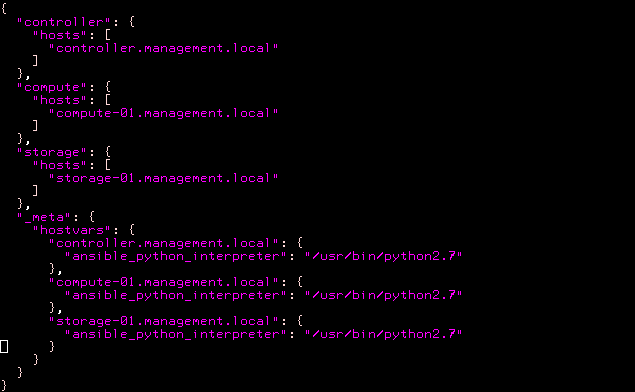
\includegraphics[scale=0.44]{img_9}
\end{frame}

\begin{frame}
  \frametitle{Inventory}

  You can specify any INI file you like by using the -i switch in the
  ansible or ansible-playbook command. Or you can specify an
  executable that generates inventory JSON with the same -i
  switch. Note that you cannot simply point at a static JSON
  file. Ansible expects the value of the -i switch to be either a
  static INI file or an executable that, when run, produces inventory
  JSON on stdout.
\end{frame}

\begin{frame}
  \frametitle{Inventory}

  Here is a trivial example. Let's write a tiny script that merely
  cats the aforementioned static JSON file:

  
\includegraphics[scale=0.44]{img_10}

  And here is an ansible command that uses it:

  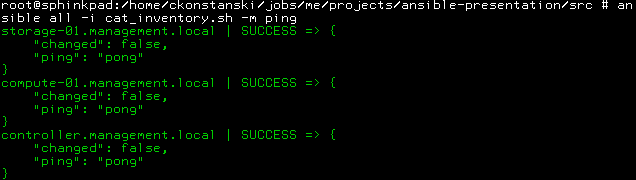
\includegraphics[scale=0.44]{img_11}

  This is a silly usage because if you were going to hardcode the
  JSON, you'd be better off hardcoding a hosts file in INI format. But
  this mechanism is incredibly useful for programatically generating
  the inventory JSON.
\end{frame}

\begin{frame}
  \frametitle{The ``all'' Target}

  Notice that the last example specified a target called
  ``all''. There is no such target group or hostname in the inventory
  JSON used in this example. What is ``all''? It is a special target
  group that means all the hosts in the inventory.
\end{frame}

\begin{frame}
  \frametitle{--extra-vars}

  You can pass in variables on the command line using the --extra-vars
  or -e switch. This is simple enough to understand that we can just
  look at the docs to learn more:

  http://docs.ansible.com/ansible/playbooks\_variables.html\#passing-variables-on-the-command-line
\end{frame}

\begin{frame}
  \frametitle{``vars'', ``with\_items'' and ``register''}

  Up until now the variable declaration methods we looked at were all
  external to the actual Ansible playbook. The remaining three ways to
  declare variables are all situated within the playbook.
\end{frame}

\begin{frame}
  \frametitle{``vars''}

  Declaring variables in the ``vars'' section of a playbook is quite
  straightforward:

  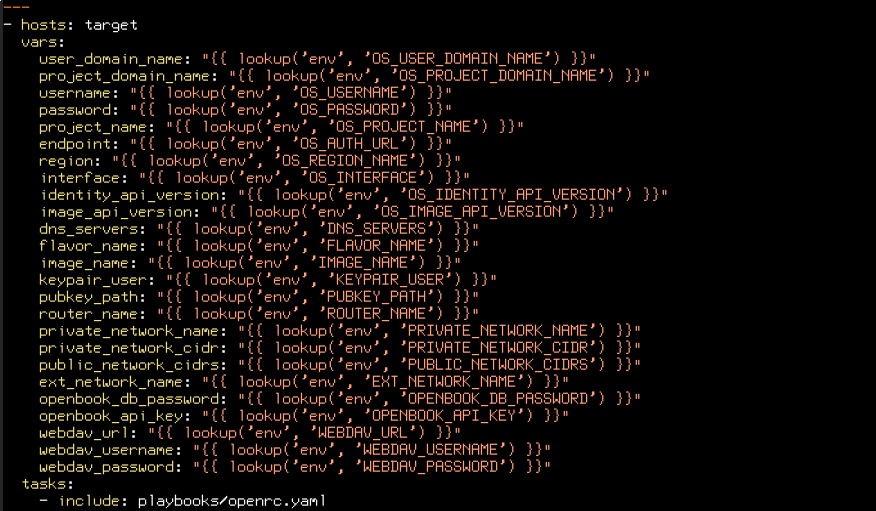
\includegraphics[scale=0.34]{img_14}
\end{frame}

\begin{frame}
  \frametitle{``with\_items''}

  ``with\_items'' is used to feed a list of values to a task. The task
  only has to be defined once and will operate on all items in the
  list.

  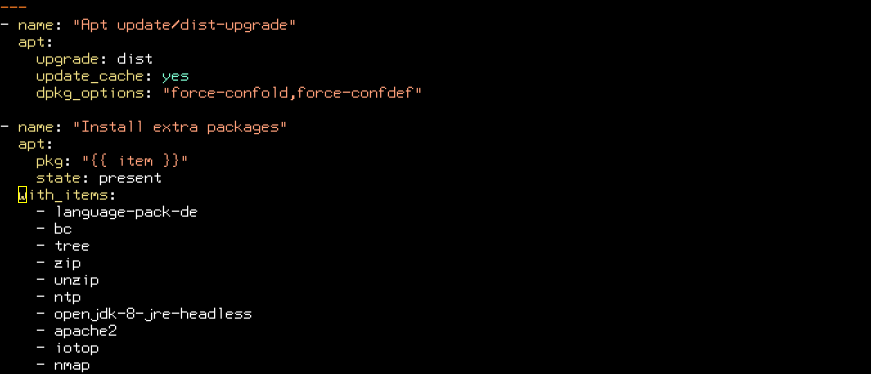
\includegraphics[scale=0.34]{img_12}
\end{frame}

\begin{frame}
  \frametitle{``with\_items''}

  The previous example used a simple list of items. ``with\_items''
  can also use hashtables. Note: this example also demonstrates the
  fact ``ansible\_hostname'' being used.

  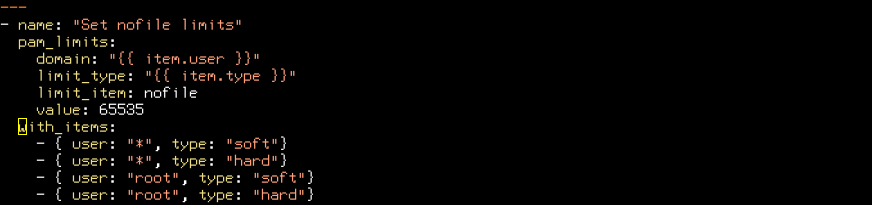
\includegraphics[scale=0.34]{img_13}
\end{frame}

\begin{frame}
  \frametitle{``register''}

  ``register'' lets you save the result of running a task into a
  variable for later use. The task needs to be one that returns
  something on stdout, most likely a shell or command resource.

  Defining a variable with ``register'' and using it in a conditional:

  
\includegraphics[scale=0.34]{img_15}
\end{frame}

\begin{frame}
  \frametitle{``register''}

  When you use ``register'' to create a variable, you don't get a
  simple scalar, but rather an entire object with many attributes. The
  example above accesses the ``changed'' attribute which holds a
  boolean value. If you use register to capture the output of a shell
  command you will most likely use the ``stdout'' or ``stdout\_lines''
  attributes.
\end{frame}

\begin{frame}
  \frametitle{Anatomy of a Playbook}

  Time to put the pieces together to understand how to write a
  complete playbook.

  Usually Ansible developers try to write playbooks in small, atomic
  units. Instead of writing one great big playbook file, they will
  write many small files and join them together with another file that
  has a bunch of ``include'' directives. The following example is from
  a playbook that provisions a Gentoo OpenStack virtual machine:

  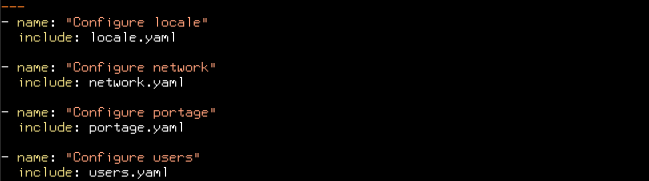
\includegraphics[scale=0.44]{img_16}
\end{frame}

\begin{frame}
  \frametitle{Anatomy of a Playbook}

  Let's look at some ``real'' playbooks (not ones containing nothing
  but includes) to begin the process of becoming comfortable with
  their contents:

  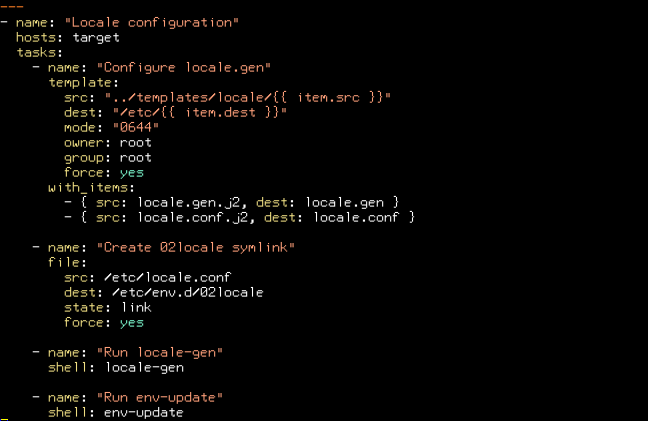
\includegraphics[scale=0.44]{img_17}
\end{frame}

\begin{frame}
  \frametitle{Anatomy of a Playbook}

  Examples continued:

  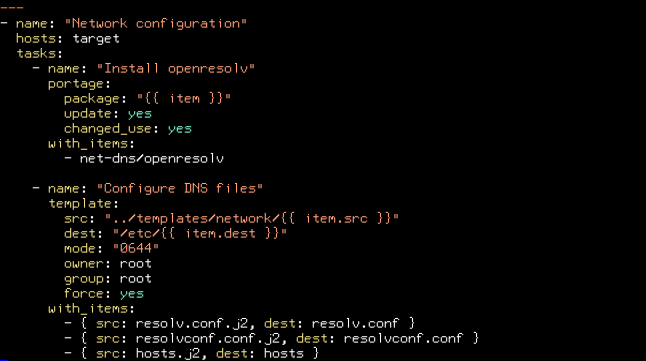
\includegraphics[scale=0.44]{img_18}
\end{frame}

\begin{frame}
  \frametitle{Anatomy of a Playbook}

  Examples continued:

  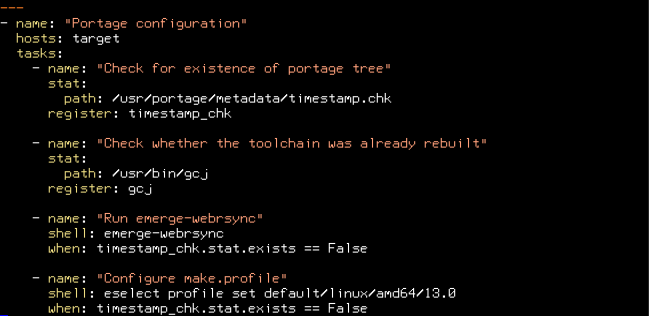
\includegraphics[scale=0.44]{img_19}
\end{frame}

\begin{frame}
  \frametitle{Writing Files}

  One of the most common tasks that configuration management systems
  must handle is the copying of files from server to target. These
  files can be categorized into two types:

  \begin{itemize}
  \item Static files (``copy'')
  \item Dynamically-generated files (``template'')
  \end{itemize}
\end{frame}

\begin{frame}
  \frametitle{Static Files}

  Use the ``copy'' resource to copy static files from the server to
  the targets. The files could be text or binary. It makes no
  difference since the contents are not processed in any way.

  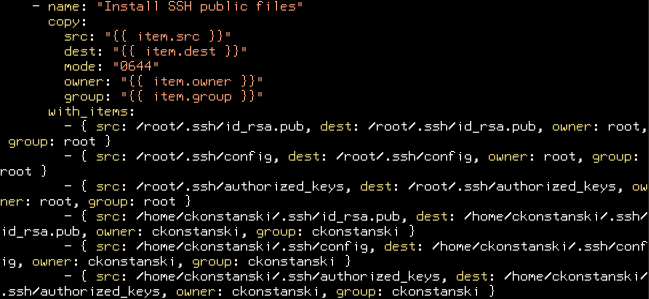
\includegraphics[scale=0.44]{img_20}
\end{frame}

\begin{frame}
  \frametitle{Dynamic Files (Templates)}

  Use the ``template'' resource to copy dynamically generated files
  from the server to the targets. The files must contain text (not
  binary files).

  The file on the server will be processed as a Jinja template. If
  there are no Jinja tags within the file, there will be no functional
  difference between it and a static file. (But the overhead of
  running it through the Jinja processing step will be a waste of
  resources.)
\end{frame}

\begin{frame}
  \frametitle{Dynamic Files (Templates)}

  An example of a playbook entry which calls the ``template'' module:

  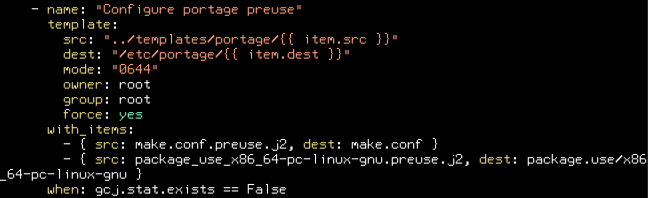
\includegraphics[scale=0.44]{img_21}
\end{frame}

\begin{frame}
  \frametitle{Dynamic Files (Templates)}

  An example of a file that is treated as a Jinja template:

  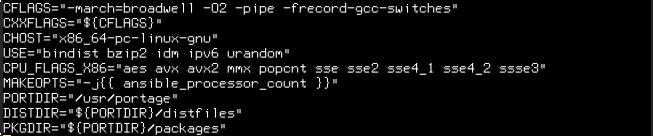
\includegraphics[scale=0.44]{img_22}
\end{frame}

\begin{frame}
  \frametitle{Packages}

  Another very common operation for configuration management to handle
  is package management.

  Usually the actions provided by a configuration management system
  are written with great pains taken to abstract away the details of
  the underlying operating system. If you want to install a package
  with Chef or Puppet, you use the ``pkg'' resource. ``pkg'' in both
  these systems is smart enough to figure out if the target is RedHat,
  Debian, Gentoo or whatever, and do the right thing accordingly with
  yum, apt or portage.

  Ansible's package management modules are not quite so smart. There
  is no ``pkg'' module. You must use the ``yum'', ``apt'' or
  ``portage'' resource and decide for yourself when it is appropriate
  to use them.
\end{frame}

\begin{frame}
  \frametitle{Packages}

  An example of installing a package on an Ubuntu system with ``apt'':

  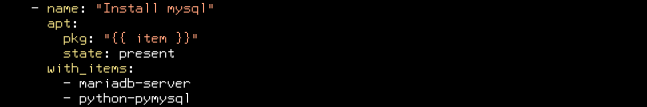
\includegraphics[scale=0.44]{img_23}
\end{frame}

\begin{frame}
  \frametitle{Packages}

  An example of installing a package on a Gentoo system with
  ``portage'':

  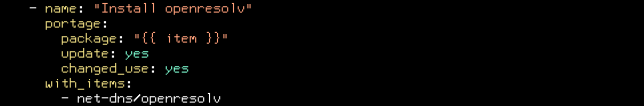
\includegraphics[scale=0.44]{img_24}
\end{frame}

\begin{frame}
  \frametitle{Services}

  The last action that we will visit is the handling of system
  services. Unlike the ill-behaved package management modules which do
  not hide the OS details, Ansible's ``service'' module works for all
  target operating systems as a proper module should.

  The following example has the extra ``runlevel'' attribute for
  Gentoo. It will throw a warning on other OSes but not cause an
  error.

  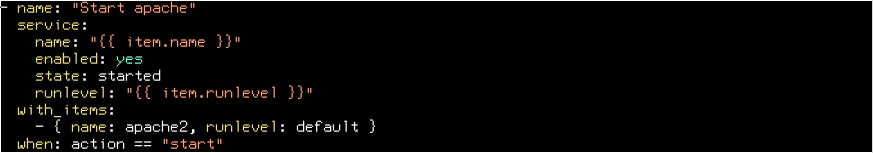
\includegraphics[scale=0.34]{img_25}
\end{frame}

\begin{frame}
  \frametitle{Orchestration}

  While we have been concentrating on Ansible's functions as a
  configuration management system, we have been neglecting its power
  as an orchestration tool. There are two playbook attributes that
  come into play for orchestration:

  \begin{itemize}
  \item ``hosts'' (to name the target(s) of the following tasks)
  \item ``serial'' (to manage whether tasks are carried out serially
    or in parallel)
  \end{itemize}
\end{frame}

\begin{frame}
  \frametitle{``hosts''}

  ``hosts'' can take the value of ``all'' (to include all known
  targets), the name of a target group, or the name of a specific
  host. Let's look at an example which uses inventory JSON (to make
  it easy to see the available targets). This is the part of the
  inventory JSON which defines the targets:

  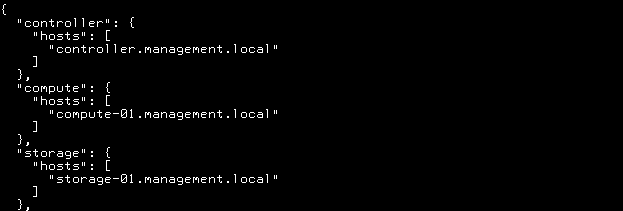
\includegraphics[scale=0.44]{img_28}
\end{frame}

\begin{frame}
  \frametitle{``hosts''}

  Now let's look at a playbook file that operates first on the
  ``controller'' target group and then the ``storage'' group. This is
  how the file starts:

  
\includegraphics[scale=0.44]{img_26}

  And in the middle we see this:

  
\includegraphics[scale=0.44]{img_27}

There are a whole set of tasks that only run on controller nodes, and
then another set of tasks that only run on storage nodes. They are
orchestrated because they execute in that order.
\end{frame}

\begin{frame}
  \frametitle{``serial''}

  Each group of tasks has a value for the number of threads it will use
  when executing. It defaults to the value of ``forks'' in
  ansible.cfg. But it can be overridden with the ``serial'' attribute
  within the playbook.

  Usually you will see ``serial: 1'' in a playbook. This is because
  the default in ansible.cfg is usually set to a high number to allow
  tasks to be performed in parallel. But there are times when tasks
  must be carried out serially, for example when building a database
  cluster.
\end{frame}

\end{document}
